% TEX compiler = pdflatex
\documentclass[12pt]{article}


\usepackage{graphicx}
\usepackage{amsmath}
\usepackage{fancyhdr}
\usepackage{geometry}
\usepackage{circuitikz}
\usepackage{subfigure}
\usepackage{caption}
\usepackage{karnaugh-map}
\usepackage{bm}
\usepackage{pst-barcode}
\usepackage[off]{auto-pst-pdf}

\geometry{letterpaper, margin=1in}
\graphicspath{ {../images/} }

% Header and Footer
\pagestyle{fancy}
\fancyhf{}
\fancyhead[L]{CSE 2301 - Lab 04: I/O and POSTNET Hardware Implementation}
\fancyhead[R]{\thepage}
\setlength{\headheight}{15pt}

\author{Arturo Salinas-Aguayo}
\title{Lab 04: Karnaugh Maps and Hardware Implementation}
% theorem set
\newtheorem{example}{Example}
% Example block environment
\newenvironment{examp}
{\vspace{0.5cm}
\hrule
\begin{example}}
{\hrule
\vspace{0.5cm}
\end{example}}

\begin{document}
\newcommand{\closure}[2][3]{%
	{}\mkern#1mu\overline{\mkern-#1mu#2}}
\newcommand\ncoverline[1]{\mkern1mu\overline{\mkern-1mu#1\mkern-1mu}\mkern1mu}
% Title Page
\begin{titlepage}
	\centering
	\vspace*{3cm}
	\huge\textbf{Lab 04: I/O and POSTNET Hardware Implementation}\\
	\vspace{5cm}
	\Large\textbf{Arturo Salinas-Aguayo}\\
	\normalsize
	CSE 2301: Principles and Practice of Digital Logic Design\\
	Dr. Mohammad Khan, Section 003L-1248\\
	Electrical and Computer Engineering Department
	\vfill
	
\includegraphics[scale=0.1]{uconnlogo}\\
	College of Engineering, University of Connecticut\\
	\scriptsize{Coded in \LaTeX}
	\vspace*{1cm}
\end{titlepage}
\section*{Theory}
\subsubsection*{Karnaugh Maps in Depth}
Looking back at last week's answer,
\begin{examp}
\vspace{3mm}
\textbf{Karnaugh Map for \(\bm{\sum m(0, 2, 3, 4, 6, 7, 8, 10, 12)}\)}
\begin{center}
\begin{karnaugh-map}(label=corner)[4][4][1][$D$][$C$][$B$][$A$]
\minterms{0,2,3,4,6,7,8,10,12}
\autoterms[0]
\implicantcorner
\implicant{3}{6}
\implicant{0}{8}
\end{karnaugh-map}
\end{center}
\textit{This produces:}
\[
	F(A,B,C,D) = \closure{A}C + \closure{B}\closure{D} + \closure{C}\closure{D}
\]
\[
	F(A,B,C,D) = \closure{A}C + \closure{D}(\closure{B} + \closure{C}) \quad \text{\textit{(Distribution)}}
\]
\end{examp}
% % ] Display an understanding of minimizing equations with Karnaugh Maps in
% your own words. How are they set up and how do you use them? Why do we
% need “don’t care” states (boxes marked with an X)?

Karnaugh maps, are a tabular, graphical way to simplify Boolean expressions by grouping terms into a grid
based on their truth tables. Each square in a K-map represents a
\textbf{minterm}, which corresponds to a \textit{unique} combination of
variable values. These minterms are placed such that adjacent squares differ
only by one variable, which allows for the user to easily identify
opportunities for simplification. These are ordered in a Grey code.

There are actually multiple ways to organize a K-map, but the most general
process involves circling adjacent squares that contain a 1, or \textbf{TRUE}
value. By grouping these \textbf{TRUE} values in the largest possible
rectangles, we can cancel out variables that appear in both true and
complimented form.

A \textbf{"Don't Care"} state is marked with an \(X\). These are used when a
certain input combination does not impact the desired output. ``Don’t care”
states, marked with an \(X\) are used when certain input combinations do not
impact the output or are not possible in the design. These states can be
treated as either 1 or 0, depending on whether they help in forming larger
groups, further reducing the complexity of the Boolean expression.

\subsubsection*{Why are "Don’t Care" states useful?}
They provide flexibility in simplifying the logic. Since their output *doesn't
matter*, they can be grouped with the 1’s to create larger rectangles, thus
reducing the number of terms in the final Boolean equation.

\subsubsection*{POSTNET (2 out of 5, 74210 weighting) and XS3:}

\begin{examp}
	\vspace{.5mm}
	\textbf{POSTNET and XS3 Encoding:}
	\vspace{.5mm}
	\begin{list}{-}{\leftmargin=1em \itemindent=0em}
		\item \textbf{POSTNET}: Postal Numeric Encoding Technique, used by the
		      U.S. Postal Service to encode ZIP codes into barcodes. It uses a
		      2-out-of-5 code where each digit is represented by five bars, and
		      exactly two of the bars are tall. The weighting used to decode
		      these bars is 74210, meaning the bars have respective weights of
		      \(7, 4, 2, 1, 0\).
		\item \textbf{XS3} (Excess-3): A binary-coded
		      decimal (BCD) system where each digit is represented by its binary
		      equivalent plus 3 (hence the term "excess-3"). For example, the
		      decimal number 5 is represented in \(XS3\) as \(0100_2\) (since 5 +
		      3 = 8 in binary).
	\end{list}
\end{examp}

\subsubsection*{Number of Non-Valid Input Codes}

To determine how many non-valid input codes are in your circuit, you need to
consider the total number of possible input combinations based on the number of
inputs. Let’s assume there are \(n\) inputs. Non-valid input codes are those combinations
that the circuit is not designed to handle or those that result in undefined behavior,
typically represented as "don't care" states in the Karnaugh map (K-map).

Given that each bit can only be either \(0\) or \(1\), there are a total of \(2^n\) possible input combinations.
For instance, if there are \(5\) inputs, there would be \(2^5 = 32\) possible combinations.
If we have specific output codes for the decimal numbers \(0\) through \(9\),
assuming these represent valid input combinations, we can calculate the number of non-valid input codes by subtracting the number of valid input codes from the total number of possible input combinations. Therefore:
\[
	\text{Number of Non-Valid Input Codes} = 2^n - 10
\]
For \(n = 5\), this would be:
\[
	\text{Number of Non-Valid Input Codes} = 32 - 10 = 22
\]

\subsection*{\textbf{POSTNET} example}
\begin{examp}
	\vspace{.3mm}
	\textbf{POSTNET} for Groton, CT
	\vspace{.5cm}
	\newline
	The ZIP code for Groton, CT is 06340-6049. This translates to:
	\begin{center}
		\begin{pspicture}(15in,10in)
			\psbarcode{063406049}{includetext}{postnet}
		\end{pspicture}
	\end{center}
\end{examp}
\newpage
\begin{examp}
	\textbf{Conversion of Binary to Ternary and Hexadecimal}\newline
	Given the binary number \( 11010010_2 \), we first convert it to decimal.
	\newline
	\textbf{Binary to Decimal}

	\[
		1 \cdot 2^7 + 1 \cdot 2^6 + 0 \cdot 2^5 + 1 \cdot 2^4 + 0 \cdot 2^3 + 0 \cdot 2^2 + 1 \cdot 2^1 + 0 \cdot 2^0 \]
	\[= 128 + 64 + 0 + 16 + 0 + 0 + 2 + 0\]
	\[= 210_{10}\]
	\newline
	\textbf{Decimal to Ternary}

	To convert decimal \(210_{10}\) to ternary, we repeatedly divide the number by 3 and record the remainders:

	\begin{center}
		\begin{tabular}{cccc}
			Dividend & Divisor & Quotient & Remainder \\
			\hline
			210      & 3       & 70       & 0         \\
			70       & 3       & 23       & 1         \\
			23       & 3       & 7        & 2         \\
			7        & 3       & 2        & 1         \\
			2        & 3       & 0        & 2         \\
		\end{tabular}
	\end{center}

	Reading the remainders from bottom to top gives \(21210_3\).
	\vspace{3mm}
	\newline
	\textbf{Decimal to Hexadecimal}

	Similarly, to convert decimal \(210_{10}\) to hexadecimal, we divide by 16:
	\begin{center}
		\begin{tabular}{cccc}
			Dividend & Divisor & Quotient & Remainder \\
			\hline
			210      & 16      & 13       & 2         \\
			13       & 16      & 0        & 13        \\
		\end{tabular}
	\end{center}

	The remainder \(13\) corresponds to hexadecimal digit \(D\), and \(2\) is itself. Therefore, the number \(210_{10}\) in hexadecimal is \(D2_{16}\).

	\textbf{Summary:}
	\begin{itemize}
		\item The binary number \(11010010_2\) converts to \(210_{10}\) in decimal.
		\item The decimal number \(210_{10}\) converts to \(21210_3\) in ternary.
		\item The decimal number \(210_{10}\) converts to \(D2_{16}\) in hexadecimal.
	\end{itemize}


\end{examp}
\begin{examp}
	Conversion of the POSTNET (9) symbol to decimal without checksum
	\begin{center}
		\begin{pspicture}(15in,10in)
			\psbarcode{937500627}{includetext}{postnet}
		\end{pspicture}
	\end{center}
\end{examp}

\begin{examp}
	\textbf{Simplifying a Logic Expression Using Boolean Logic Theorems}

	\textbf{Given Formula:}

	\[ \closure{D}(C\closure{B} + \closure{A}) + \overline{\closure{D} + A} \]

	\[ \closure{D}(C\closure{B} + \closure{A}) + \closure{\closure{D}}\closure{A} \quad \text{(Demorgan's Theorem)}\]

	\[ \closure{D}(C\closure{B} + \closure{A}) + D\closure{A}  \quad \text{(Involution)}\]

	\[ \closure{D}C\closure{B} +\closure{D}\closure{A} + D\closure{A}  \quad \text{(Distribution)}\]

	\[ \closure{D}C\closure{B} +\closure{A}(\closure{D}+ D) \quad \text{(Distributive Law)}\]

	\textbf{Final Answer:}

	\[ \closure{D}C\closure{B} +\closure{A} \quad \text{(Complement Law)}\]
	\begin{center}
		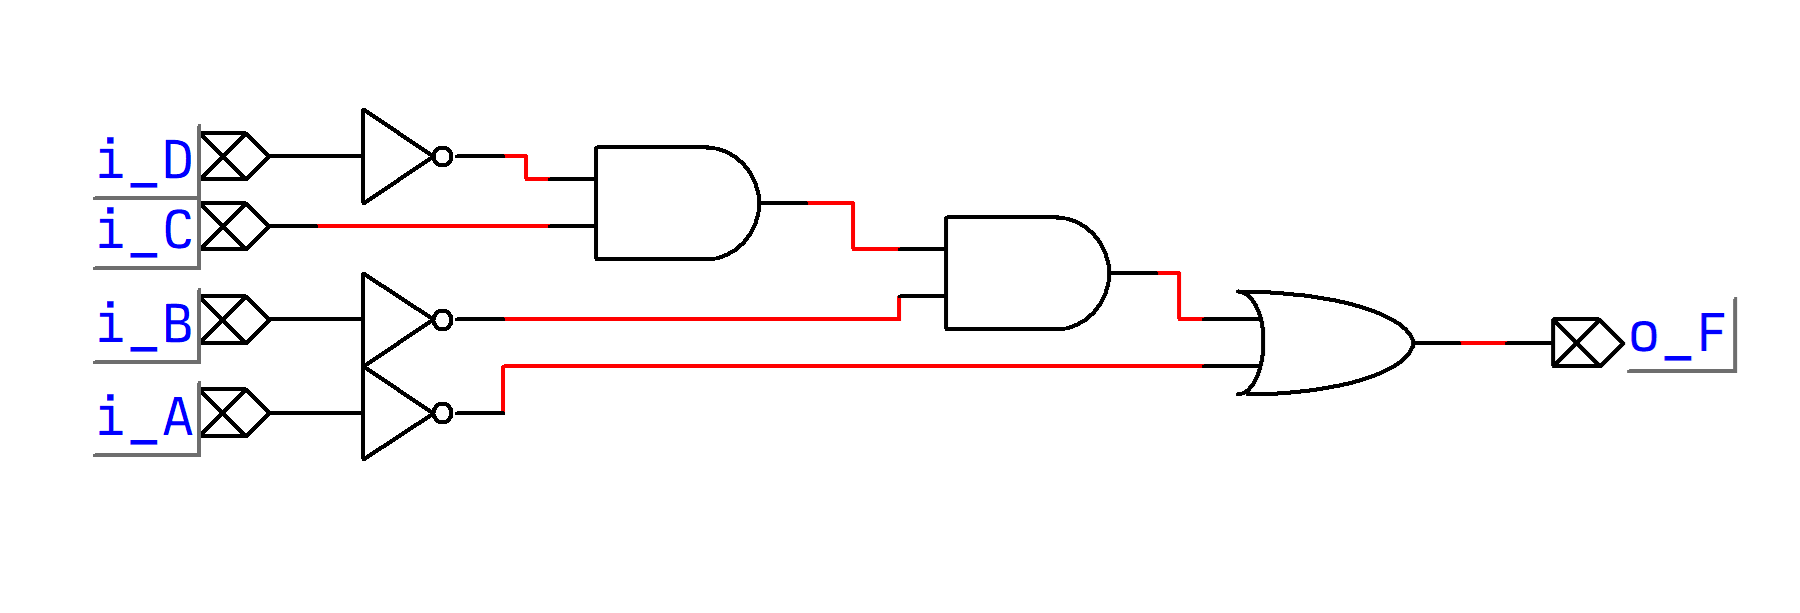
\includegraphics[scale=0.3]{lab043}
	\end{center}

\end{examp}

\end{document}
% vim: set spell spelllang=en_us expandtab tabstop=4 shiftwidth=4 softtabstop=4:
=======
\documentclass[12pt]{article}

\usepackage{graphicx}
\usepackage{amsmath}
\usepackage{fancyhdr}
\usepackage{geometry}
\usepackage{circuitikz}
\usepackage{subfigure}
\usepackage{caption}
\usepackage{karnaugh-map}
\usepackage{bm}
\usepackage{pst-barcode}
\usepackage{auto-pst-pdf}

\geometry{letterpaper, margin=1in}
\graphicspath{ {../images/} }

% Header and Footer
\pagestyle{fancy}
\fancyhf{}
\fancyhead[L]{CSE 2301 - Lab 04: I/O and POSTNET Hardware Implementation}
\fancyhead[R]{\thepage}
\setlength{\headheight}{15pt}

\author{Arturo Salinas-Aguayo}
\title{Lab 04: Karnaugh Maps and Hardware Implementation}
% theorem set
\newtheorem{example}{Example}
% Example block environment
\newenvironment{examp}
{\vspace{0.5cm}
\hrule
\begin{example}}
{\hrule
\vspace{0.5cm}
\end{example}}

\begin{document}
\newcommand{\closure}[2][3]{%
	{}\mkern#1mu\overline{\mkern-#1mu#2}}
\newcommand\ncoverline[1]{\mkern1mu\overline{\mkern-1mu#1\mkern-1mu}\mkern1mu}
% Title Page
\begin{titlepage}
	\centering
	\vspace*{3cm}
	\huge\textbf{Lab 04: I/O and POSTNET Hardware Implementation}\\
	\vspace{5cm}
	\Large\textbf{Arturo Salinas-Aguayo}\\
	\normalsize
	CSE 2301: Principles and Practice of Digital Logic Design\\
	Dr. Mohammad Khan, Section 003L-1248\\
	Electrical and Computer Engineering Department
	\vfill
	
\includegraphics[scale=0.1]{uconnlogo}\\
	College of Engineering, University of Connecticut\\
	\scriptsize{Coded in \LaTeX}
	\vspace*{1cm}
\end{titlepage}
\section*{Theory}
\subsubsection*{Karnaugh Maps in Depth}
Looking back at last week's answer,
\begin{examp}
\vspace{3mm}
\textbf{Karnaugh Map for \(\bm{\sum m(0, 2, 3, 4, 6, 7, 8, 10, 12)}\)}
\begin{center}
\begin{karnaugh-map}(label=corner)[4][4][1][$D$][$C$][$B$][$A$]
\minterms{0,2,3,4,6,7,8,10,12}
\autoterms[0]
\implicantcorner
\implicant{3}{6}
\implicant{0}{8}
\end{karnaugh-map}
\end{center}
\textit{This produces:}
\[
	F(A,B,C,D) = \closure{A}C + \closure{B}\closure{D} + \closure{C}\closure{D}
\]
\[
	F(A,B,C,D) = \closure{A}C + \closure{D}(\closure{B} + \closure{C}) \quad \text{\textit{(Distribution)}}
\]
\end{examp}
% % ] Display an understanding of minimizing equations with Karnaugh Maps in
% your own words. How are they set up and how do you use them? Why do we
% need “don’t care” states (boxes marked with an X)?

Looking back through the example, we can see that Karnaugh maps, are a tabular,
graphical way to simplify Boolean expressions by grouping terms into a grid
based on their truth tables. Each square in a K-map represents a
\textbf{minterm}, which corresponds to a \textit{unique} combination of
variable values. These minterms are placed such that adjacent squares differ
only by one variable, which allows for the user to easily identify
opportunities for simplification. These are ordered in a Grey code.

There are actually multiple ways to organize a K-map, but the most general
process involves circling adjacent squares that contain a 1, or \textbf{TRUE}
value. By grouping these \textbf{TRUE} values in the largest possible
rectangles, we can cancel out variables that appear in both true and
complimented form.

A \textbf{"Don't Care"} state is marked with an \(X\). These are used when a
certain input combination does not impact the desired output. ``Don’t care”
states, marked with an \(X\) are used when certain input combinations do not
impact the output or are not possible in the design. These states can be
treated as either 1 or 0, depending on whether they help in forming larger
groups, further reducing the complexity of the Boolean expression.

\subsubsection*{Why are "Don’t Care" states useful?}
They provide flexibility in simplifying the logic. Since their output doesn't
matter, they can be grouped with the 1’s to create larger rectangles, thus
reducing the number of terms in the final Boolean equation.

\subsubsection*{POSTNET (2 out of 5, 74210 weighting) and XS3:}

\begin{examp}
	\vspace{.5mm}
	\textbf{POSTNET and XS3 Encoding:}
	\vspace{.5mm}
	\begin{list}{-}{\leftmargin=1em \itemindent=0em}
		\item \textbf{POSTNET}: Postal Numeric Encoding Technique, used by the
		      U.S. Postal Service to encode ZIP codes into barcodes. It uses a
		      2-out-of-5 code where each digit is represented by five bars, and
		      exactly two of the bars are tall. The weighting used to decode
		      these bars is 74210, meaning the bars have respective weights of
		      \(7, 4, 2, 1, 0\).
		\item \textbf{XS3} (Excess-3): A binary-coded
		      decimal (BCD) system where each digit is represented by its binary
		      equivalent plus 3 (hence the term "excess-3"). For example, the
		      decimal number 5 is represented in \(XS3\) as \(0100_2\) (since 5 +
		      3 = 8 in binary).
	\end{list}
\end{examp}

\subsubsection*{Number of Non-Valid Input Codes:}

To determine how many non-valid input codes are in your circuit, you need to
consider the total number of possible input combinations based on the number of
inputs (let’s assume $nn$ inputs). The total number of input combinations is
$2n2n$. Non-valid input codes are those combinations that the circuit is not
designed to handle or those that result in undefined behavior, typically
represented as "don’t care" states in the K-map.

For instance, if you have 4 inputs, the total number of possible combinations
is \(2^4 = 16\). If you are only using $12$, then there would be \(16 - 12 =
16 - 12  = 4\)  non-valid input codes.
\subsection*{\textbf{POSTNET} example}
\begin{examp}
	\vspace{.3mm}
	\textbf{POSTNET} for Groton, CT
	\vspace{.5cm}
	\begin{center}
		\begin{pspicture}(15in,10in)
			\psbarcode{06340}{includetext}{postnet}
		\end{pspicture}
	\end{center}
\end{examp}
\end{document}
% vim: set spell spelllang=en_us expandtab tabstop=4 shiftwidth=4 softtabstop=4:
>>>>>>> Stashed changes
